\documentclass{article}
\usepackage[utf8]{inputenc}
\usepackage{kotex}
\usepackage{amsmath}
\usepackage{graphicx}
\usepackage{subfigure}
\usepackage{verbatim}

\title{2022 Data Structure HW12}
\author{TaeYong Kim (C011060)}
\date{\today}

\begin{document}

\maketitle

\section{Class 설계 내용 및 이유}

다음은 AVL 트리의 구현하기 위한 class 설계 내용들이다.

\begin{verbatim}
struct Node {
    int height;
    int key;

    nodeptr data;
    Node* leftChild;
    Node* rightChild;
};

class bstree {
public:
    Node* insert(const int value, Node*& root);
    void show(Node* root) ;
    void search(const int key, Node* root);
    Node* del(const int key, Node* root);
};
\end{verbatim}

\subsection{Node}
Node는 struct 형이다. 노드의 높이를 할당하는 height와 노드의 key를 담고 있는 key가 있다. 그리고 nodeptr인 data와 Node*형인 leftChild와 rightChild를 가지고 있다.

\subsection{bstree}
bstree는 class 형이다. tree에 노드를 추가하는 Node*형 insert 함수와 tree에 노드를 삭제하는 Node*형 del 함수, 경로를 탐색하는 void형 search 함수와 tree의 내용을 보여주는 void형 show 함수가 있다.

\section{AVL Tree의 연산들 설명}

다음은 AVL 트리의 연산을 하는 함수들이다.

\begin{verbatim}
nodeptr RotateLeft(nodeptr x) {
    nodeptr y = x->rightChild;
    x->rightChild = y->leftChild;
    y->leftChild = x;

    x->height = std::max(getHeight(x->leftChild), getHeight(x->rightChild)) + 1;
    y->height = std::max(getHeight(y->leftChild), getHeight(y->rightChild)) + 1;

    return y;
}

nodeptr RotateRight(nodeptr y) {
    nodeptr x = y->leftChild;
    y->leftChild = x->rightChild;
    x->rightChild = y;

    y->height = std::max(getHeight(y->leftChild), getHeight(y->rightChild)) + 1;
    x->height = std::max(getHeight(x->leftChild), getHeight(x->rightChild)) + 1;

    return x;
}

void Balancing(nodeptr &r, int item) {
    int bF = getBalanceFactor(r);

    // left left
    if (bF > 1 && getBalanceFactor(r->leftChild) >= 0) {
        r = RotateRight(r);
    }
    // left right
    else if (bF > 1 && getBalanceFactor(r->leftChild) < 0) {
        r->leftChild = RotateLeft(r->leftChild);
        r = RotateRight(r);
    }
    // right right
    else if (bF < -1 && getBalanceFactor(r->rightChild) <= 0) {
        r = RotateLeft(r);
    }
    // right left
    else if (bF < -1 && getBalanceFactor(r->rightChild) > 0) {
        r->rightChild = RotateRight(r->rightChild);
        r = RotateLeft(r);
    }
}
\end{verbatim}

\subsection{Rotate Left}
Rotate Left(왼쪽으로 회전) 기능은 x에 루트를 둔 하위 트리를 왼쪽으로 회전시킨다. x의 오른쪽 자식, 즉 y를 하위 트리의 새 루트로 만들고 x를 y의 왼쪽 자식으로 만들어 이를 수행한다. 이것은 tree의 균형을 유지하기 위함이다.

\subsection{Rotate Right}
Rotate Right 함수도 비슷하게 하위 트리의 새 루트인 y의 왼쪽 자식을 x로 만들고 y를 x의 오른쪽 자식으로 만들어 하위 트리를 오른쪽으로 회전시킨다.

\subsection{Balancing}
Balancing 함수는 노드를 삽입하거나 삭제한 후 트리의 균형을 조정하는 데 사용된다. 좌우 child인 루트 노드의 Balance Factor를 확인하고 적절한 회전을 수행하여 트리의 밸런스를 맞춘다. Balance Factor가 1보다 크면 왼쪽 child가 오른쪽 child보다 height가 크므로 left-left 또는 left-right 회전이 필요할 수 있습니다. Balance Factor를이 -1 미만이면 오른쪽 child가 왼쪽 child보다  height가 크고 오른쪽 또는 오른쪽 왼쪽 회전이 필요하다.

\subsection{getHeight}
getHeight 함수는 노드에서 가장 깊은 leaf까지의 edge 수인 지정된 노드의 높이를 반환합니다. getBalanceFactor 함수는 지정된 노드의 Balance Factor를 반환합니다. 이는 왼쪽 및 오른쪽 하위 노드의 높이 차이이다. 이러한 함수는 트리의 균형과 회전이 필요한지 여부를 결정하는 데 사용된다.

\begin{verbatim}
Node* bstree::insert(const int value, Node*& root) {
    if (root == nullptr) {
        nodeptr z = new Node;
        z->key = value;
        root = z;
        return root;
    } else if (root->key < value) {
        root->rightChild = insert(value, root->rightChild);
    } else {
        root->leftChild = insert(value, root->leftChild);
    }

    root->height = std::max(getHeight(root->leftChild), getHeight(root->rightChild)) + 1;

    Balancing(root, value);
    return root;
};

Node* bstree::del(const int key, Node* root) {
    if (root == nullptr)
        return root;

    if (key < root->key)
        del(key, root->rightChild);

    else if (key > root->key)
        del(key, root->rightChild);

    else {
        if (root->leftChild == nullptr) {
            Node* temp = root->rightChild;
            delete root;
            root = temp;
        } else if (root->rightChild == nullptr) {
            Node* temp = root->leftChild;
            delete root;
            root = temp;
        } else {
            Node* temp = minNode(root->rightChild);
            root->key = temp->key;
            del(temp->key, root->rightChild);
        }
    }
    if (root == NULL)
        return root;

    root->height = std::max(getHeight(root->leftChild), getHeight(root->rightChild)) + 1;
    Balancing(root, key);
    return root;
}

void bstree::search(const int key, Node* root) {
    if (root == NULL)
        return;

    std::cout << root->key;

    if (root->key == key)
        return;

    // If the key is less than the current node, search the left subtree
    if (key < root->key) {
        std::cout << "->";
        search(key, root->leftChild);
    }
        
    // If the key is greater than the current node, search the right subtree
    else if (key > root->key) {
        std::cout << "->";
        search(key, root->rightChild);
    }
}
\end{verbatim}

\subsection{insert}
insert 함수는 AVL 트리의 삽입 연산을 수행하는 함수이다..
AVL 트리는 균형 잡힌 이진 트리의 일종으로, 삽입 연산을 수행할 때마다 균형을 유지할 수 있도록 자식 노드의 깊이 차이가 2 이하가 되도록 균형을 잡는다.

코드의 첫 번째 if 문은 root가 nullptr인 경우를 처리한다. 이 경우에는 새로운 노드를 생성해 값을 삽입하고, root를 새로 생성한 노드로 설정한다.
그 다음 else if 문과 else 문은 value가 root의 키보다 작은 경우와 큰 경우를 처리한다. 이 경우에는 재귀 호출을 이용해 적절한 위치에 삽입할 수 있도록 한다.
그 후에 root의 height값을 재설정합니다. height값은 왼쪽 자식 노드와 오른쪽 자식 노드의 height값 중 큰 값에 1을 더한 값이다.
마지막으로 Balancing 함수를 호출해 균형을 잡는다.

\subsection{delete}
delete 함수는 AVL 트리의 삭제 연산을 수행하는 함수이다.
AVL 트리는 균형 잡힌 이진 트리의 일종으로, 삭제 연산을 수행할 때마다 균형을 유지할 수 있도록 자식 노드의 깊이 차이가 2 이하가 되도록 균형을 잡는다.

코드의 첫 번째 if 문은 root가 nullptr인 경우를 처리합니다. 이 경우에는 root를 그대로 반환한다.
그 다음 else if 문과 else 문은 key가 root의 키보다 작은 경우와 큰 경우, 그리고 같은 경우를 처리한다. 이 경우에는 재귀 호출을 이용해 적절한 위치에서 삭제할 수 있도록 한다.
삭제할 노드가 자식 노드가 없거나 자식 노드가 하나인 경우에는 그냥 삭제하고, 자식 노드가 두 개인 경우에는 삭제할 노드의 오른쪽 서브트리에서 가장 작은 값을 가지는 노드를 찾아 삭제할 노드를 삭제한다. 마지막으로 Balancing 함수를 호출해 균형을 잡는다.

\subsection{search}
search 함수는 AVL 트리에서 특정 값을 가지는 노드를 경로를 출력하는 연산을 수행하는 함수이다.
AVL 트리는 이진 탐색 트리의 일종이기 때문에, 탐색 연산은 이진 탐색 트리의 기본적인 구조를 이용한다.

코드의 첫 번째 if 문은 root가 nullptr인 경우를 처리합니다. 이 경우에는 아무것도 하지 않고 함수를 종료한다.
그 다음 cout 문은 root의 키 값을 출력한다.
그 후에 if 문과 else if 문은 key가 root의 키보다 작은 경우와 큰 경우를 처리한다. 이 경우에는 재귀 호출을 이용해 적절한 위치에서 탐색을 수행할 수 있도록 한다.

\section{결과 값(출력) 및 결과 분석}

\subsection{실행 예시 1}
그림\ref{ex1}은 search, add, delete, show 기능을 보여주는 그림이다. \\

(1) 첫번째 기능은 search 기능으로, 노드를 입력하면 root부터 입력 노드까지의 path를 보여준다. \\

(2) add 기능은 새로운 노드를 입력하면 Balance Factor가 균형있게 tree에 추가가 된다. 그리고 추가된 노드를 포함된 tree를 출력한다. \\

(3) delete 기능은 입력된 노드를 삭제한다. 마찬가지로 Balance Factor가 균형있게 삭제된다. \\

\subsection{실행 예시 2}
본 실행의 초기 값을 그림으로 표현하면 \ref{tree-1}으로 표현된다. 

(1) add node "2":
그림\ref{ex2-1}는 노드 "2"를 추가했을 때의 출력이다. 이를 그림으로 표현하면 그림 \ref{tree-2}으로 표현된다.

(2) add node "9", "11":
그림\ref{ex2-2}는 노드 "9"와 "11"을 순차적으로 추가했을 때의 출력이다. 이를 그림으로 표현하면 그림 \ref{tree-3}으로 표현된다.

(3) delete node "19":
그림\ref{ex2-1}는 노드 "19"를 삭제했을 때의 출력이다. 이를 그림으로 표현하면 그림 \ref{tree-4}으로 표현된다.

\begin{figure}
\centering
   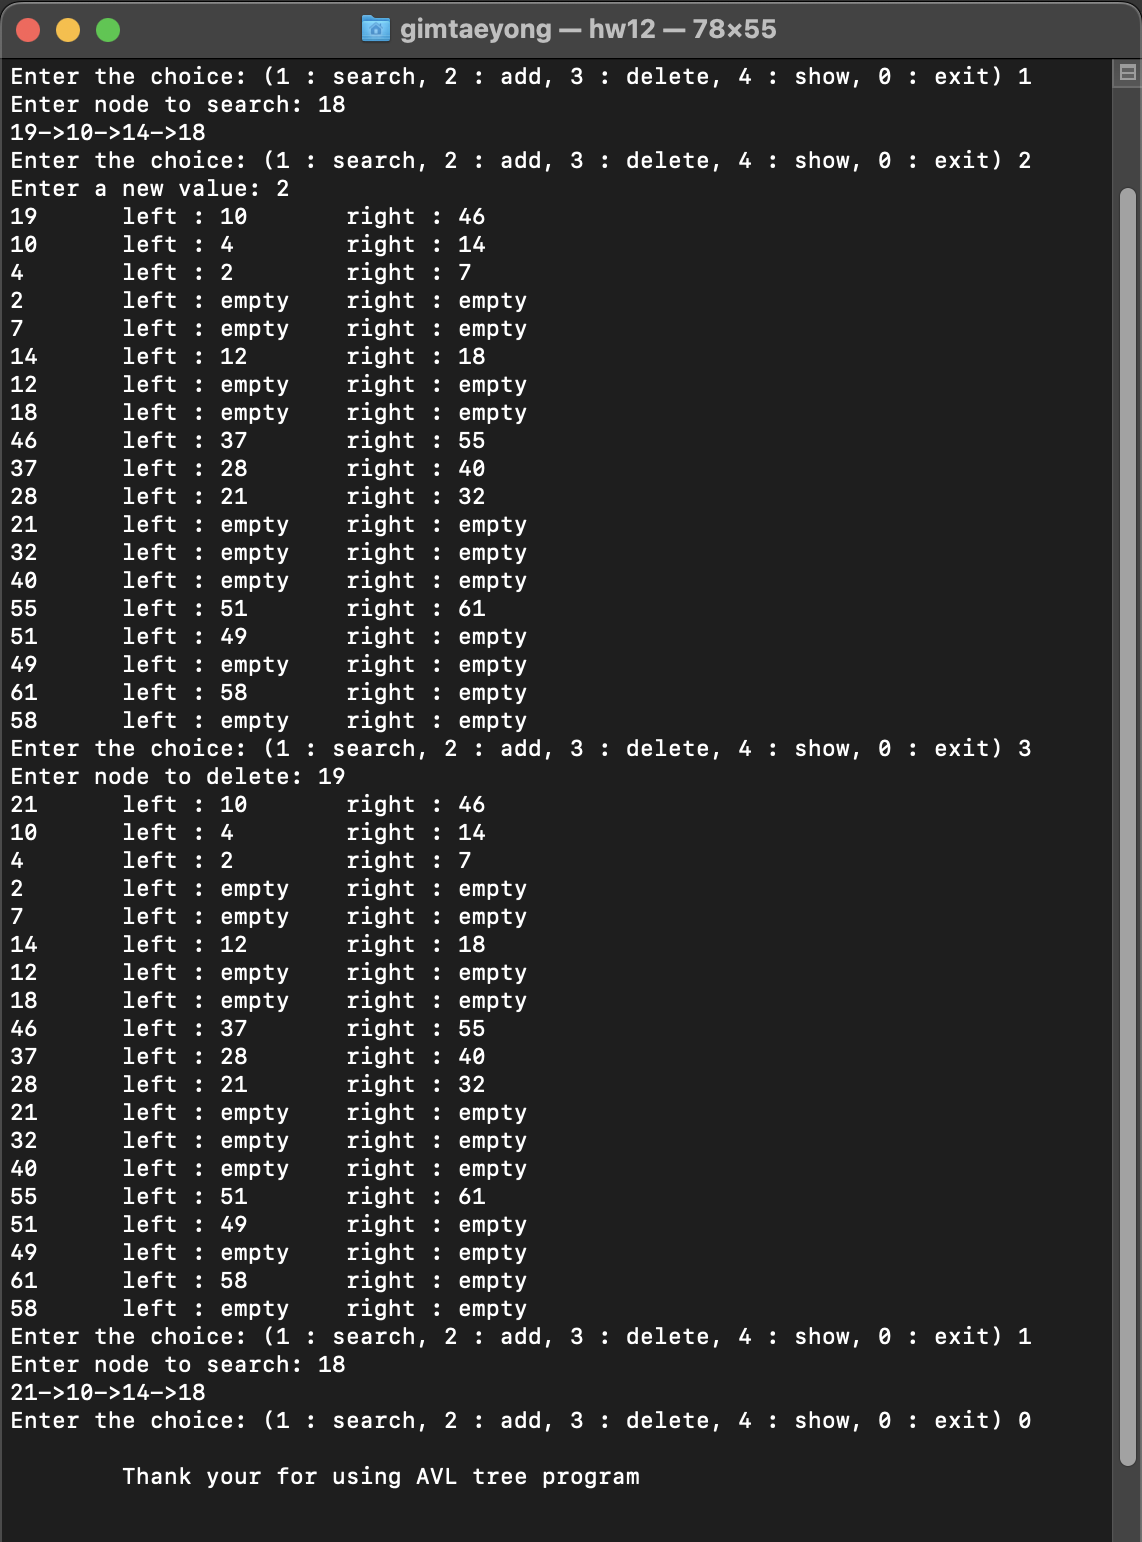
\includegraphics[width=11cm]{ex_1.png}
   \hfil
\caption{실행 예시 1 결과 값}
\label{ex1}
\end{figure}

\begin{figure}
\centering
   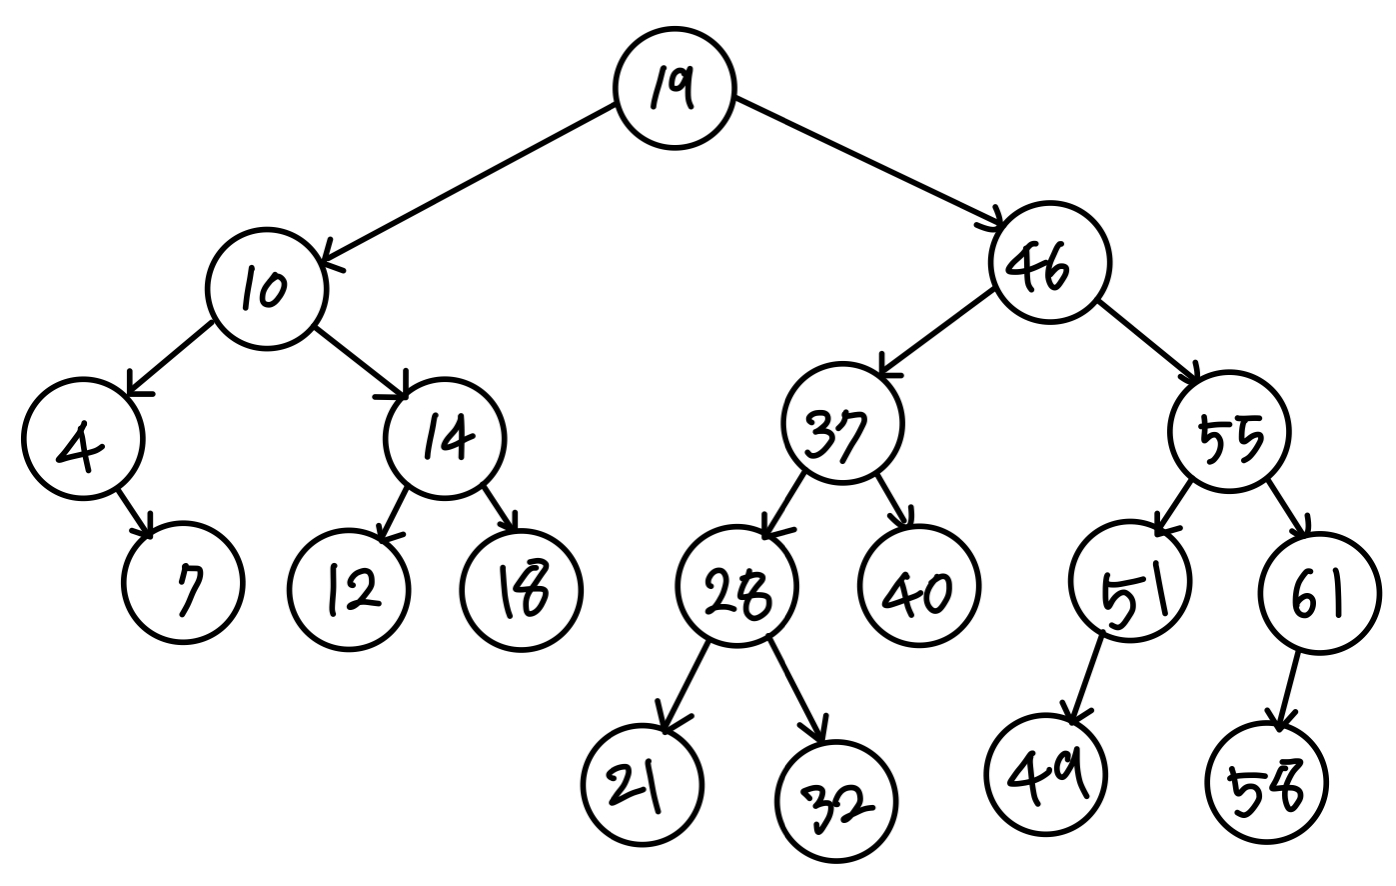
\includegraphics[width=11cm]{tree-1.jpeg}
   \hfil
\caption{실행 예시 2의 초기 트리}
\label{tree-1}
\end{figure}

\begin{figure}
\centering
   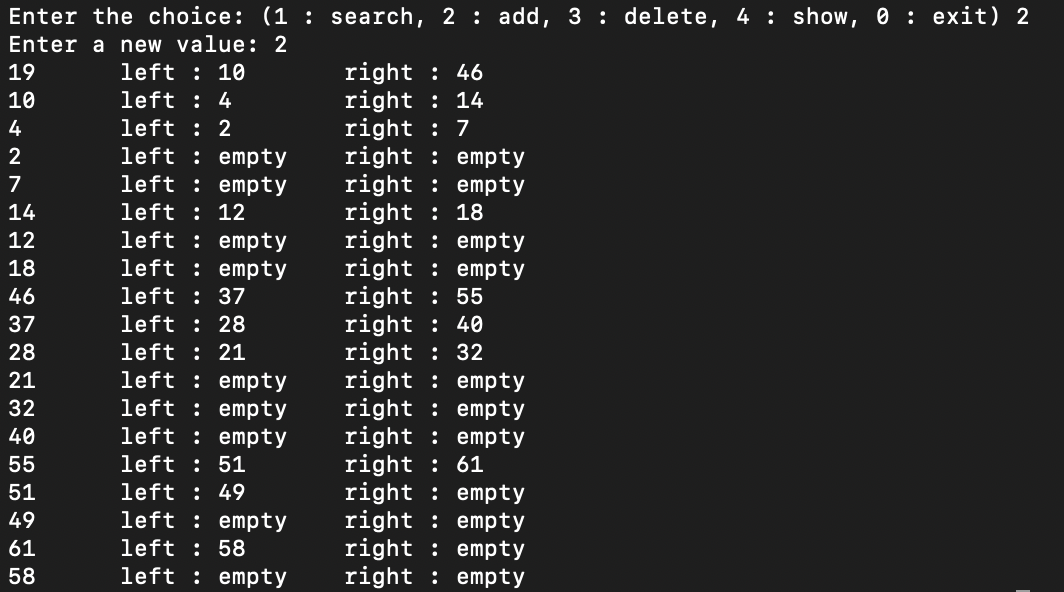
\includegraphics[width=11cm]{ex_2-1.png}
   \hfil
\caption{실행 예시 2-1 결과 값}
\label{ex2-1}
\end{figure}

\begin{figure}
\centering
   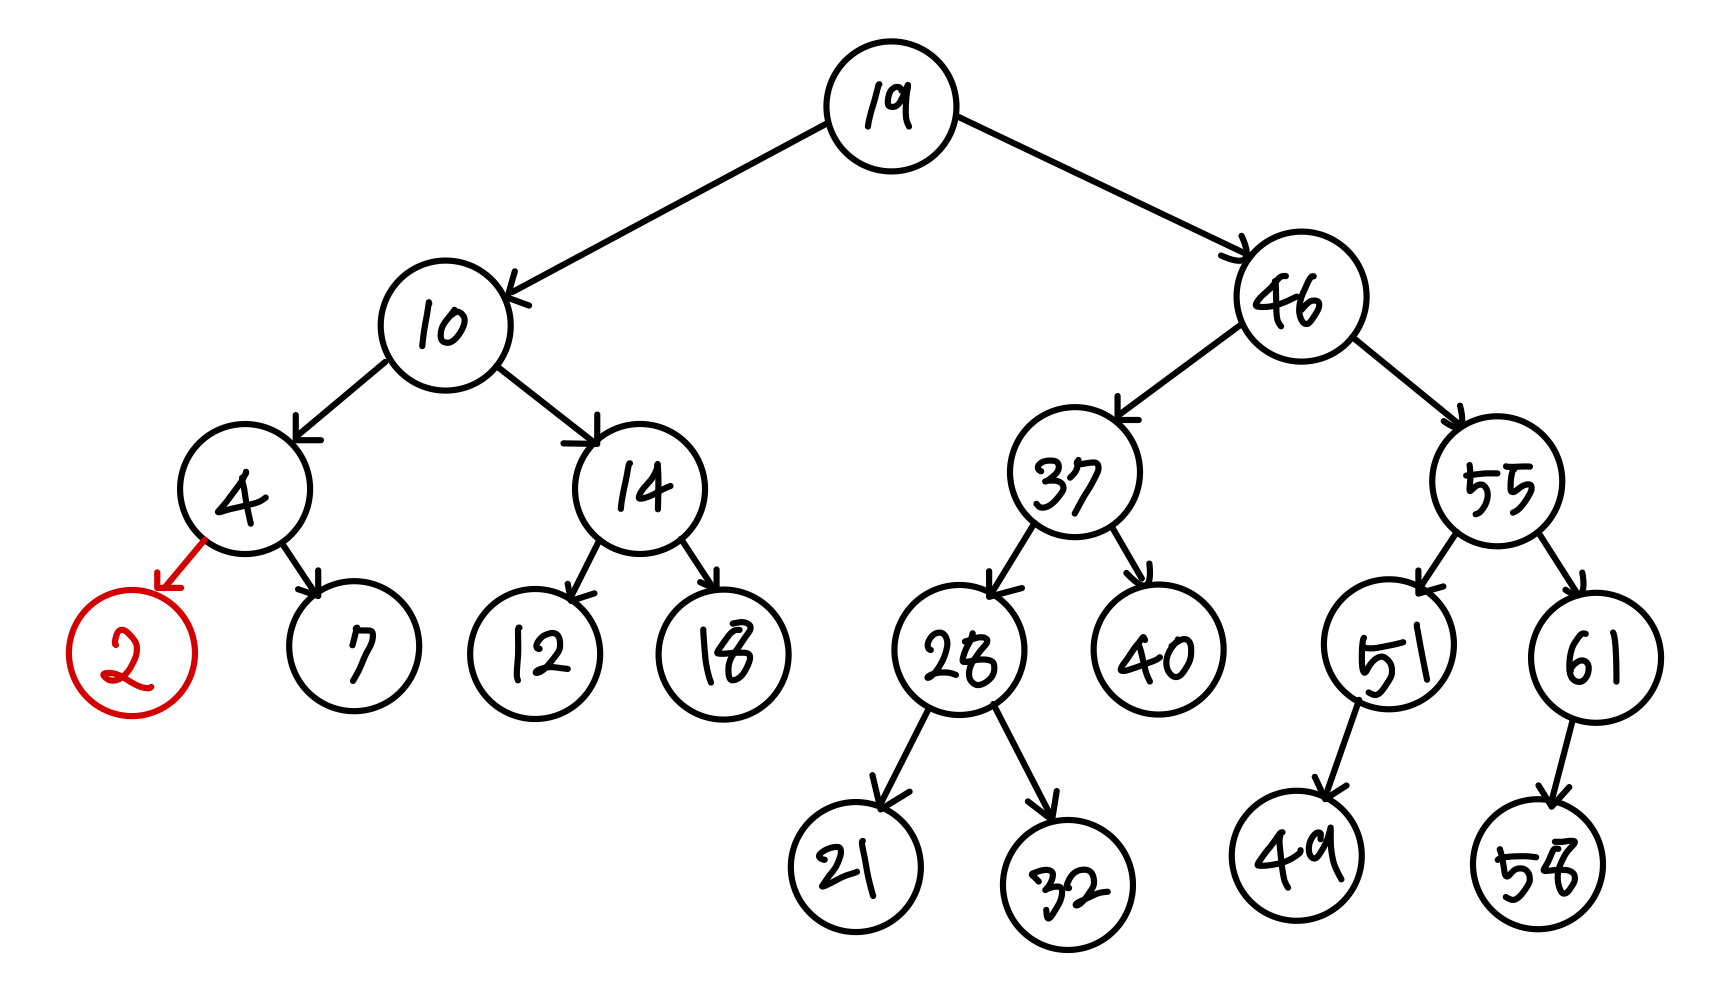
\includegraphics[width=11cm]{tree-2.jpeg}
   \hfil
\caption{실행 예시 2-1 결과 트리}
\label{tree-2}
\end{figure}

\begin{figure}
\centering
   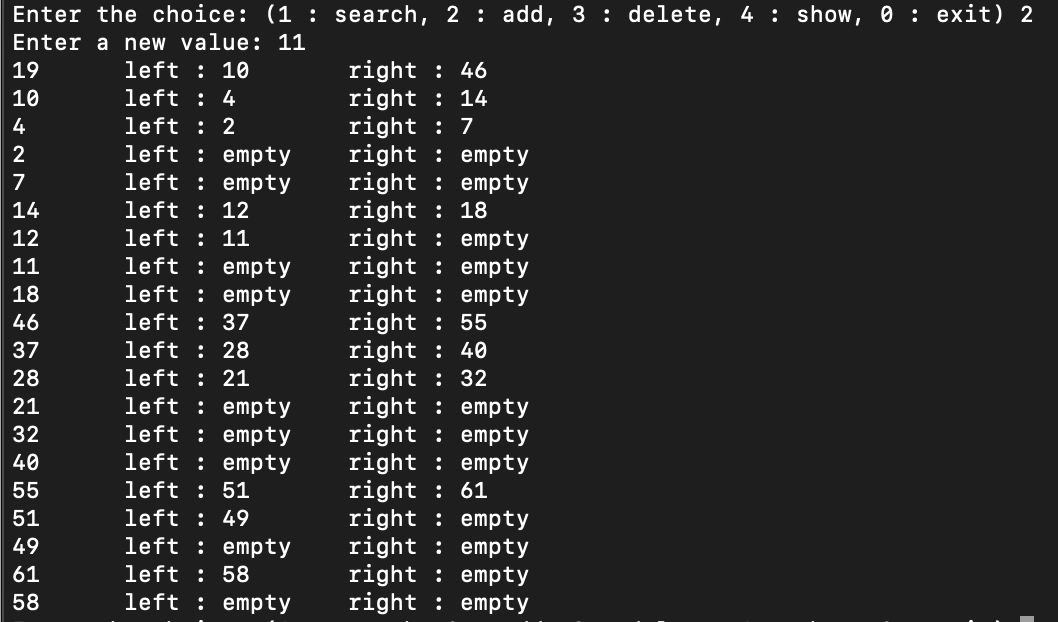
\includegraphics[width=11cm]{ex_2-2.png}
   \hfil
\caption{실행 예시 2-2 결과 값}
\label{ex2-2}
\end{figure}

\begin{figure}
\centering
   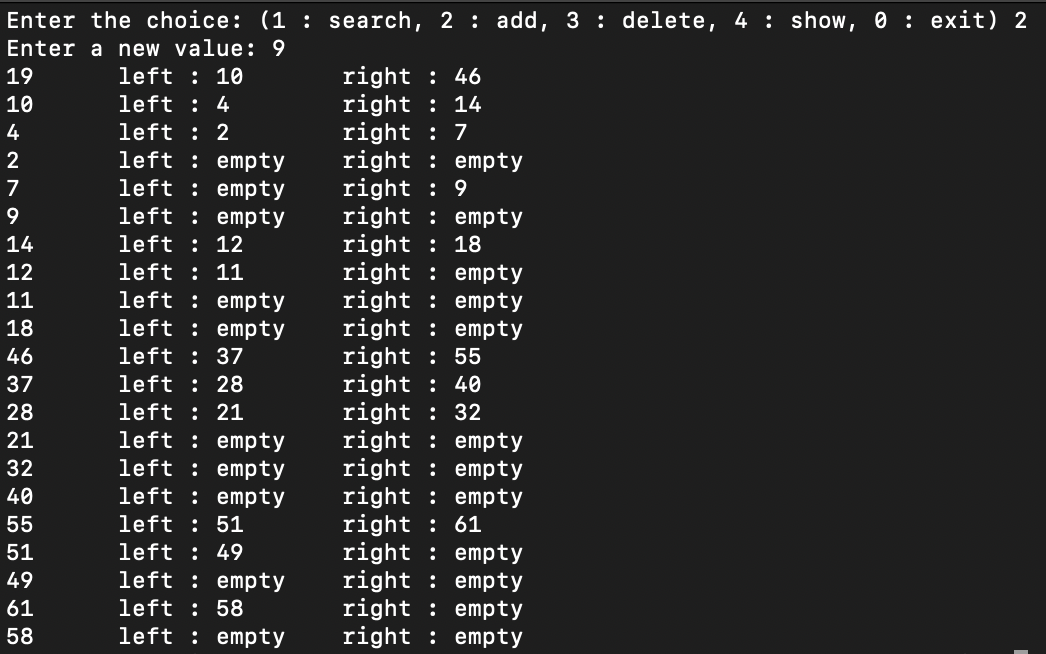
\includegraphics[width=11cm]{ex_2-3.png}
   \hfil
\caption{실행 예시 2-3 결과 값}
\label{ex2-3}
\end{figure}

\begin{figure}
\centering
   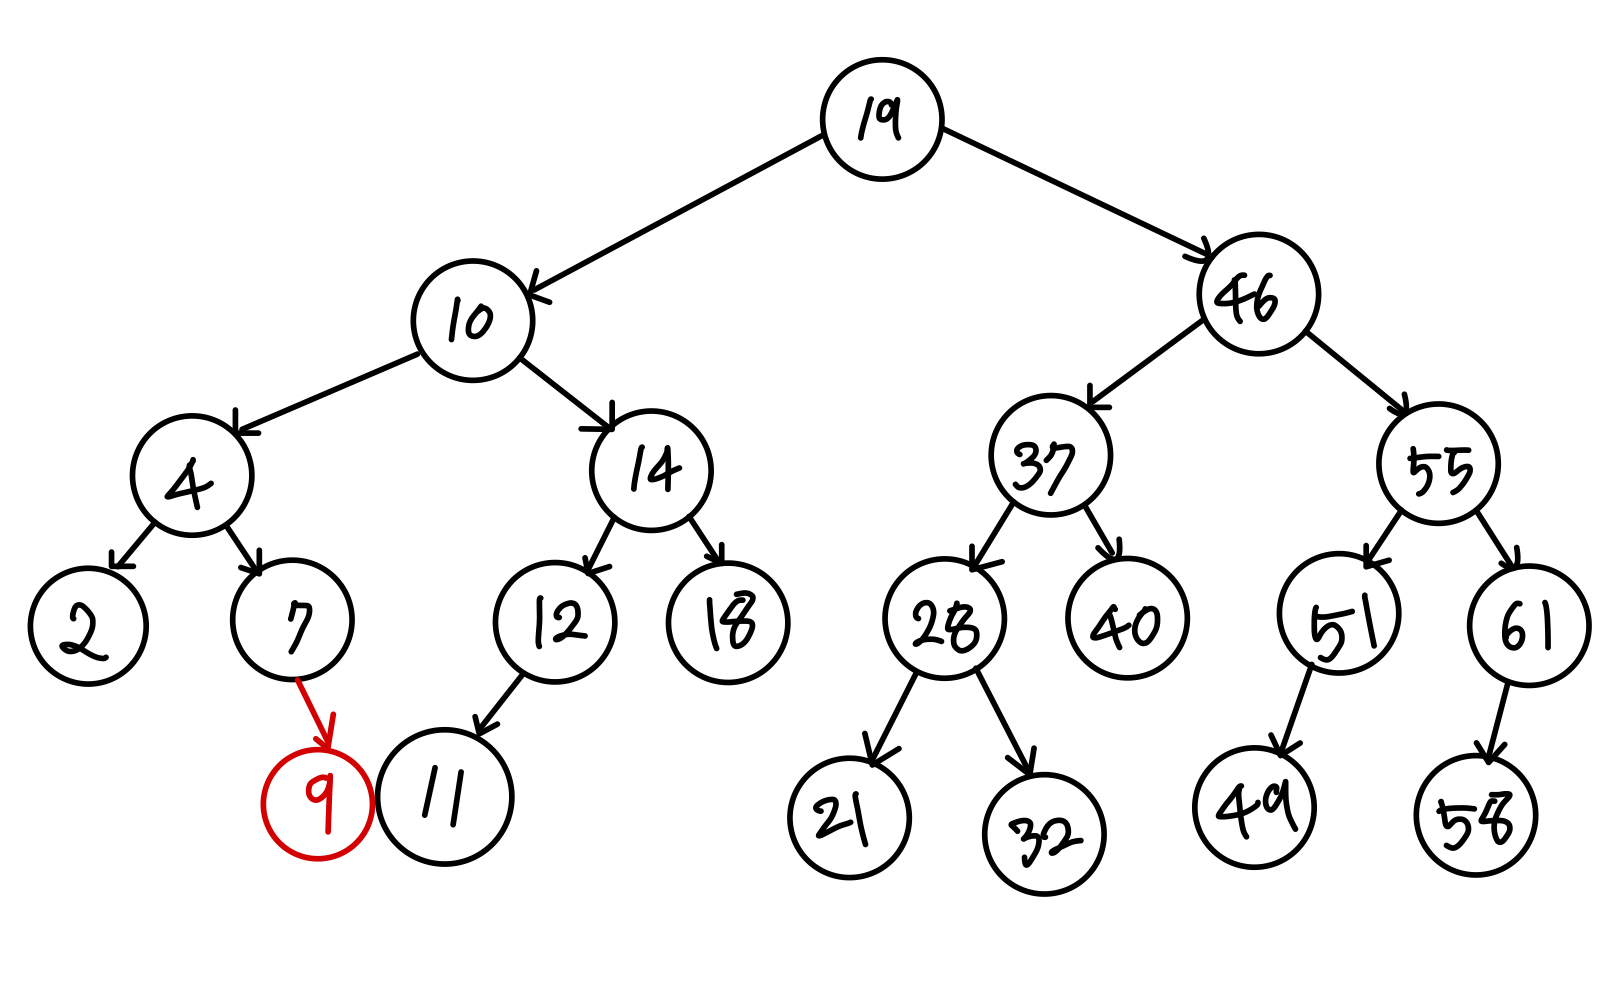
\includegraphics[width=11cm]{tree-3.jpeg}
   \hfil
\caption{실행 예시 2-2/2-3 결과 트리}
\label{tree-3}
\end{figure}


\begin{figure}
\centering
   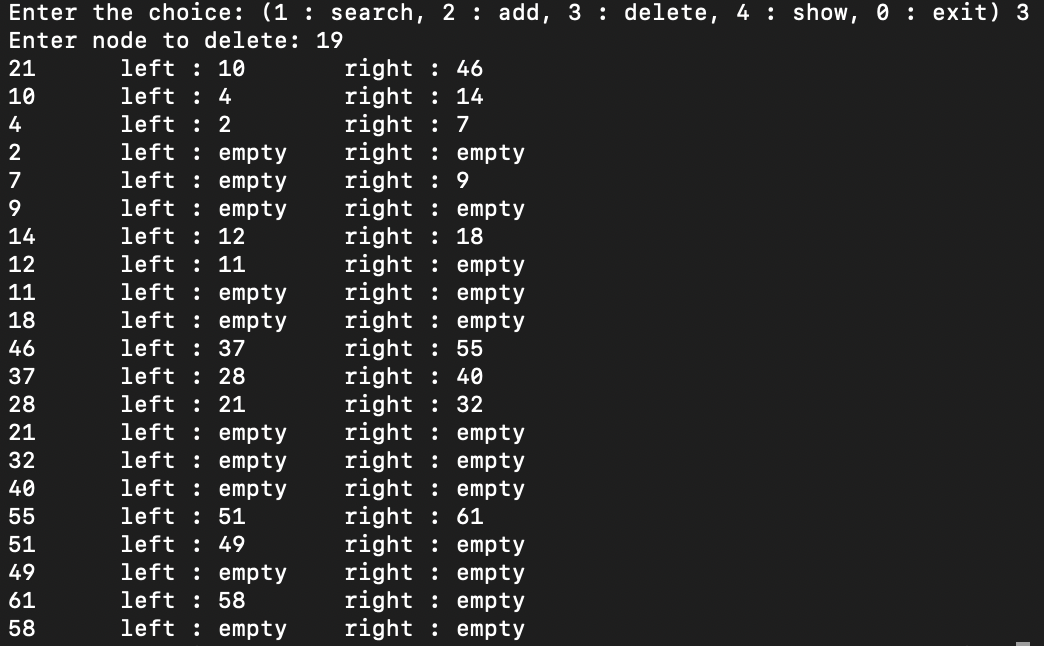
\includegraphics[width=11cm]{ex_2-4.png}
   \hfil
\caption{실행 예시 2-4 결과 값}
\label{ex2-4}
\end{figure}

\begin{figure}
\centering
   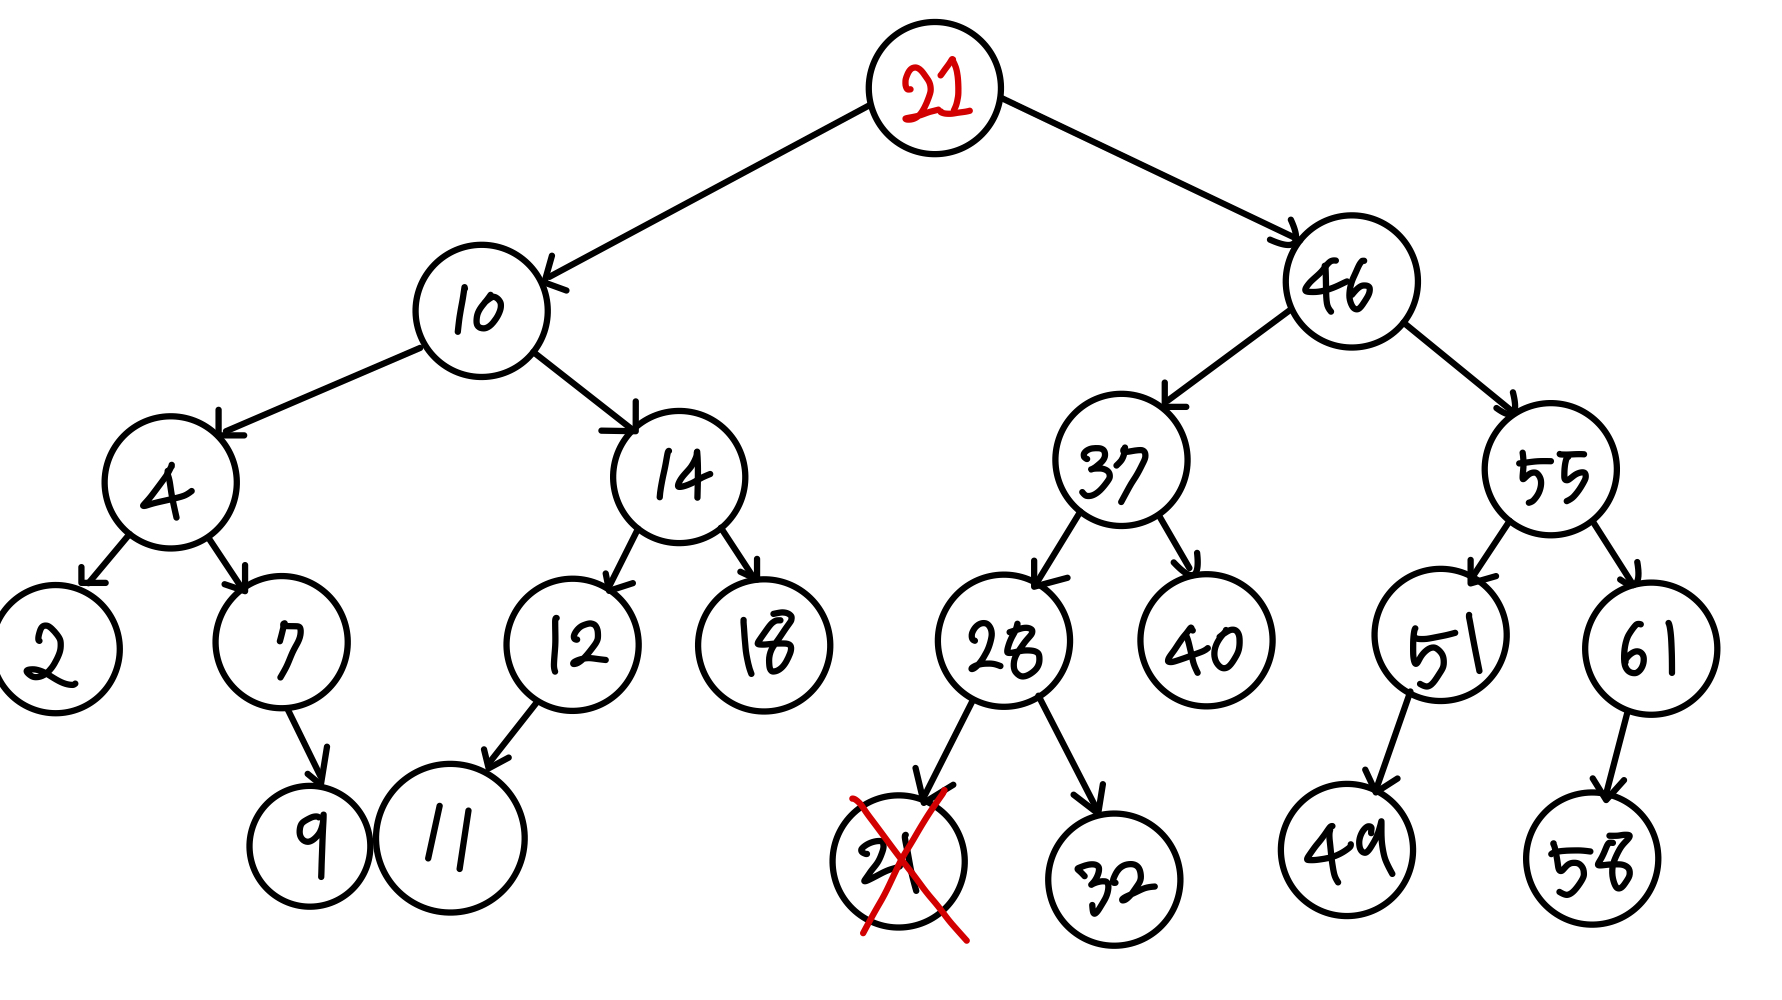
\includegraphics[width=11cm]{tree-4.jpeg}
   \hfil
\caption{실행 예시 2-4 결과 트리}
\label{tree-4}
\end{figure}


\end{document}

